\documentclass[12pt, titlepage]{article}

\usepackage{booktabs}
\usepackage{tabularx}
\usepackage{hyperref}
\usepackage{graphicx}
\usepackage{longtable}
\usepackage[utf8]{inputenc}
\usepackage[T1]{fontenc}
\usepackage{lmodern}
\usepackage{parskip}
\hypersetup{
    colorlinks,
    citecolor=black,
    filecolor=black,
    linkcolor=red,
    urlcolor=blue
}

\usepackage[round]{natbib}

%% Comments

\usepackage{color}

\newif\ifcomments\commentstrue %displays comments
%\newif\ifcomments\commentsfalse %so that comments do not display

\ifcomments
\newcommand{\authornote}[3]{\textcolor{#1}{[#3 ---#2]}}
\newcommand{\todo}[1]{\textcolor{red}{[TODO: #1]}}
\else
\newcommand{\authornote}[3]{}
\newcommand{\todo}[1]{}
\fi

\newcommand{\wss}[1]{\authornote{blue}{SS}{#1}} 
\newcommand{\plt}[1]{\authornote{magenta}{TPLT}{#1}} %For explanation of the template
\newcommand{\an}[1]{\authornote{cyan}{Author}{#1}}

%% Common Parts

\newcommand{\progname}{ProgName} % PUT YOUR PROGRAM NAME HERE
\newcommand{\authname}{Team \#, Team Name
\\ Student 1 name
\\ Student 2 name
\\ Student 3 name
\\ Student 4 name} % AUTHOR NAMES                  

\usepackage{hyperref}
    \hypersetup{colorlinks=true, linkcolor=blue, citecolor=blue, filecolor=blue,
                urlcolor=blue, unicode=false}
    \urlstyle{same}
                                


\begin{document}

\title{Verification and Validation Report: \progname} 
\author{\authname}
\date{\today}
	
\maketitle

\pagenumbering{roman}

\section{Revision History}

\begin{tabularx}{\textwidth}{p{3cm}p{2cm}X}
\toprule {\bf Date} & {\bf Version} & {\bf Notes}\\
\midrule
Date 1 & 1.0 & Notes\\
Date 2 & 1.1 & Notes\\
\bottomrule
\end{tabularx}

~\newpage

\section{Symbols, Abbreviations and Acronyms}

\renewcommand{\arraystretch}{1.2}
\begin{tabular}{l l} 
  \toprule		
  \textbf{symbol} & \textbf{description}\\
  \midrule 
  TPG & Tangled Program Graphs\\
  DNNs & Deep Neural Networks\\
  RL & Reinforcement Learning\\
  SRS & Software Requirement Specification\\
  FR & Functional Requirement\\
  NFR & Non-Functional Requirement\\
  SLN & System Level Number\\
  VnV & Verification and Validation\\
  \bottomrule
\end{tabular}\\

% \wss{symbols, abbreviations or acronyms -- you can reference the SRS tables if needed}

\newpage

\tableofcontents

\listoftables %if appropriate

\listoffigures %if appropriate

\newpage

\pagenumbering{arabic}

This document cohesively summarizes the results of each test as specified in the \href{https://github.com/TPGEngine/tpg/blob/main/docs/VnVPlan/VnVPlan.pdf}{VnV Plan} documentation.

\section{Functional Requirements Evaluation}

\subsection{MuJoCo Integration}
\label{mujoco_integration}

\begin{center}
\begin{longtable}{|p{2cm}|p{8cm}|p{2cm}|}
  \caption{MuJoCo Integration Tests} \\
\hline
\textbf{Test Id} & \textbf{Notes} & \textbf{Result} \\
\hline
\endfirsthead
\hline
\textbf{Test Id} & \textbf{Notes} & \textbf{Result} \\
\hline
\endhead
FR-SLN1 & When executing the appropriate script, all MuJoCo environments can be run. The best-performing agent within the policy can be visualized using OpenGL or an MP4 file. & Pass \\
\hline
FR-SLN2 & MuJoCo environments within the TPG framework can be successfully run within the Digital Research Alliance, enabling research to be conducted by executing experiments. & Pass \\
\hline
\end{longtable}
\end{center}

\subsection{Experiment Visualization}
\label{experiment_visualization}

\begin{center}
  \begin{longtable}{|p{2cm}|p{8cm}|p{2cm}|}
    \caption{Experiment Visualization Tests} \\
  \hline
  \textbf{Test Id} & \textbf{Notes} & \textbf{Result} \\
  \hline
  \endfirsthead
  \hline
  \textbf{Test Id} & \textbf{Notes} & \textbf{Result} \\
  \hline
  \endhead
  FR-SLN3 & When an experiment is running or finished training, the best performing policy can be visualized using the TPG CLI tool. & Pass \\
  \hline
  \end{longtable}
\end{center}

\subsection{Github Actions CI/CD Pipeline}
\label{github_actions}

\subsection{Software Engineering Practices}
\label{software_engineering_practices}

\begin{center}
  \begin{longtable}{|p{2cm}|p{8cm}|p{2cm}|}
    \caption{Software Engineering Practices Tests} \\
  \hline
  \textbf{Test Id} & \textbf{Notes} & \textbf{Result} \\
  \hline
  \endfirsthead
  \hline
  \textbf{Test Id} & \textbf{Notes} & \textbf{Result} \\
  \hline
  \endhead
  FR-SLN6 & Newly added code in the TPG codebase follows Google's C++ Style Guide and software engineering best practices such as design patterns, and object-oriented design. This includes careful review and consideration of code readability, extendability, maintainability and scalability. A linter has also been implemented to check for such styling as discussed in \ref{github_actions}. & Pass \\
  \hline
  \end{longtable}
\end{center}

\section{Nonfunctional Requirements Evaluation}

\subsection{Usability}
\begin{center}
  \begin{longtable}{|p{4cm}|p{4cm}|}
  \caption{Usability Tests} \\
  \hline
  \textbf{Test Id} & \textbf{Result} \\
  \hline
  \endfirsthead
  \hline
  \textbf{Test Id} & \textbf{Result} \\
  \hline
  \endhead
  NFR-SLN1 & Pass \\
  \hline
  NFR-SLN2 & Pass \\
  \hline
  NFR-SLN3 & Pass \\
  \hline
  \end{longtable}
\end{center}

For NFR-SLN1, the TPG framework now includes comprehensive documentation across multiple levels. The main README provides installation instructions and a quick start guide, while the CLI tool documentation details commands for evolving, plotting, and replaying policies. Code documentation with inline comments explains classes and methods, and YAML configuration files include detailed parameter descriptions. Usability testing with graduate students confirmed the documentation's effectiveness, with a rating of 10/10 for installation experience.

For NFR-SLN2, an event-driven logging architecture was implemented to provide real-time, accurate message logging throughout the training process. Metrics are stored in CSV files, capturing timing, selection, replacement, and removal data. The CLI tool provides real-time feedback during experiment execution. Usability testing rated the accuracy and usefulness of system logs at 9/10, with suggestions to clarify CSV file naming conventions and document the meaning of removal and replacement metrics in the wiki.

For NFR-SLN3, the framework now offers extensive customization options for MuJoCo simulation parameters through YAML configuration files. Each environment includes specific parameters (reward weights, health criteria, observation settings) and common simulation parameters (maximum timesteps, model path). The CLI tool integrates these parameters, allowing users to specify different environments and configurations when running experiments. Usability testing confirmed the ease of locating and customizing parameters, with suggestions to place YAML files within the experiments directory and reduce the number of log files.
		
\subsection{Performance}

\begin{center}
  \begin{longtable}{|p{4cm}|p{4cm}|}
  \caption{Performance Tests} \\
  \hline
  \textbf{Test Id} & \textbf{Result} \\
  \hline
  \endfirsthead
  \hline
  \textbf{Test Id} & \textbf{Result} \\
  \hline
  \endhead
  NFR-SLR4 & Pass \\
  \hline
  \end{longtable}
\end{center}

For NFR-SLN4, test cases within TPG for the experimental environments have been implemented to check for the accuracy of the numerical computations associated during training. Declaration of variables with proper types (e.g. signed long or int, unsigned long or int) has also been taken into consideration to reduce issues in the future for extremely large or small numbers that may overflow. TPG has been comprehensively tested to guarantee that all computations with high numerical precision (e.g. during the runtime of an experiment) are accurate and contain an acceptable tolerance limit of 0.00001. The results were inspected manually by comparing the actual output to the anticipated output, and performing a calculation to check for quantitative error, and if such error meets the requirements for numerical precision.

\begin{figure}[h]
  \centering
  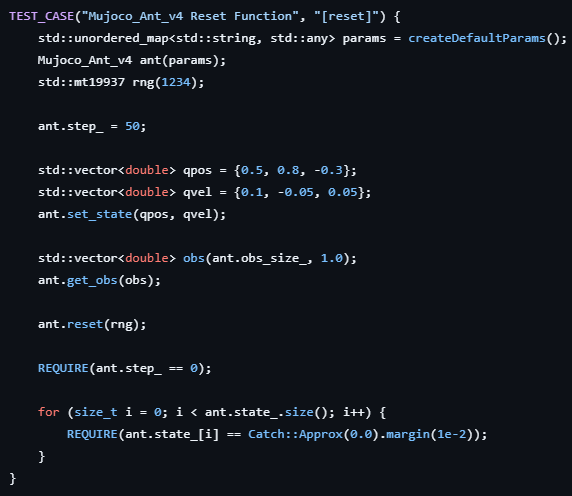
\includegraphics[width=1\textwidth]{img/ant_test.png}
  \caption{Example of a Numerical Computation Test}
  \label{fig:myimage}
\end{figure}

\subsection{Operational and Environmental}

\begin{center}
  \begin{longtable}{|p{4cm}|p{4cm}|}
  \caption{Operational and Environmental Tests} \\
  \hline
  \textbf{Test Id} & \textbf{Result} \\
  \hline
  \endfirsthead
  \hline
  \textbf{Test Id} & \textbf{Result} \\
  \hline
  \endhead
  NFR-SLR6 & Pass \\
  \hline
  \end{longtable}
\end{center}

For NFR-SLN6, TPG now supports contributions from macOS, Windows, and Linux developers.
Previously, only Linux was supported because TPG used SCons for C++ builds and Linux-specific dependencies from \href{https://gitlab.cas.mcmaster.ca/kellys32/tpg/-/blob/main/requirements.txt}{requirements.txt}.
With VSCode Dev Containers, a Linux development environment is automatically launched for all developers, ensuring a standardized setup.
Simply follow the \href{https://gitlab.cas.mcmaster.ca/kellys32/tpg/-/wikis/home}{Wiki} instructions to download all necessary Linux dependencies and build the C++ code reliably. Onboarding on a Macbook has been reduced from 2 weeks to just 5 minutes.

\subsection{Maintainability}

\subsection{Security}

\begin{center}
  \begin{longtable}{|p{4cm}|p{4cm}|}
  \caption{Security Tests} \\
  \hline
  \textbf{Test Id} & \textbf{Result} \\
  \hline
  \endfirsthead
  \hline
  \textbf{Test Id} & \textbf{Result} \\
  \hline
  \endhead
  NFR-SLR8 & Pass \\
  \hline
  \end{longtable}
\end{center}

For NFR-SLN8, the .csv, .txt, .png and .mp4 files that are generated within Classic Control and MuJoCo experiments are ignored by Git when making commits to the public repositories in GitHub and GitLab to reduce chance of oversharing sensitive data. Currently, none of these files generate sensitive data, but to follow best practice and to keep the repository at a clean state, these are not recognized when synchronizing code to each respective repository. Additionally, the team has also manually checked all stored .csv, .txt, .png and .mp4 files along with others that may contain textual information to see if data within them are sensitive and must be kept private. 

\subsection{Compliance}

\begin{center}
\begin{longtable}{|p{4cm}|p{4cm}|}
\caption{Compliance Tests} \\
\hline
\textbf{Test Id} & \textbf{Result} \\
\hline
\endfirsthead
\hline
\textbf{Test Id} & \textbf{Result} \\
\hline
\endhead
NFR-SLR9 & Pass \\
\hline
\end{longtable}
\end{center}

The modified codebase is successfully analyzed using Clang-Tidy and Clang-Format within the CI/CD pipeline. 
Code change discussions take place through pull request conversations made to the main branch. 
All errors and warnings are generated based on the C++ Style Guidelines. 
Any critical errors found during the linting process create blocking pull request conversations that must be resolved before merging into the main branch.

\begin{figure}[h]
  \centering
  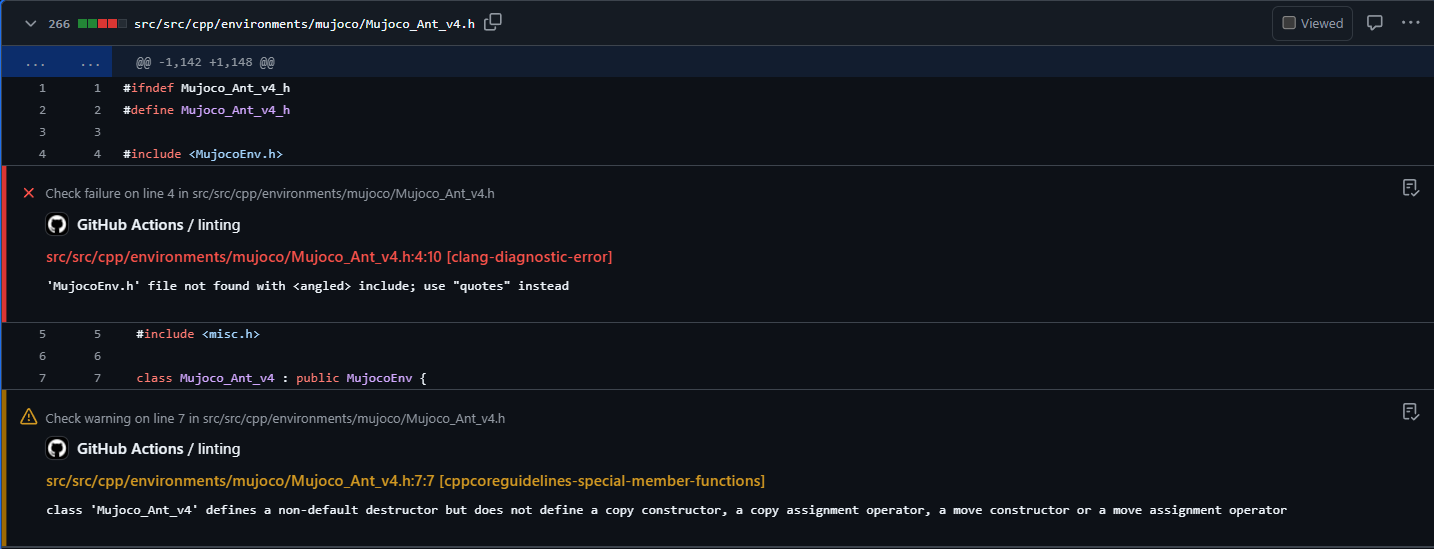
\includegraphics[width=1\textwidth]{img/linter-example.png}
  \caption{Example of a Linter Error}
  \label{fig:myimage}
\end{figure}

\section{Unit Testing}

\section{Changes Due to Testing}

% \wss{This section should highlight how feedback from the users and from 
% the supervisor (when one exists) shaped the final product.  In particular 
% the feedback from the Rev 0 demo to the supervisor (or to potential users) 
% should be highlighted.}
\subsection{Feedback from Rev 0}
The feedback given by the instructor and teaching assistant during Revision 0 was essential in guiding the next steps as the team looks toward the final demonstration.
Emphasis was placed on ensuring that usability testing was executed systematically rather than in the more ad-hoc manner initially planned by the team.
Some additional changes to be made include ensuring that unit testing and benchmarking of the implemented environments are cohesively executed and investigating whether the integration of deployment within the DRA is possible.

\section{Automated Testing}

As a result of the team’s conversion from building the project using SCons to CMake, automated testing became significantly easier to execute and debug.
To run any automated tests within a developer’s local environment, a developer can simply execute a command to build the project. 
This not only compiles everything but also runs all automated tests. If a developer wishes to run only the tests, they must navigate to the directory where the tests were already compiled (typically \texttt{/build/tests}). 
From there, the command \texttt{ctest} can be entered into the command prompt. Similar to the compilation process, all automated tests are executed once this command is run.\\

From the repository’s point of view, tests are executed using GitHub Actions or GitLab CI (depending on which repository is being viewed). 
Both linting and compilation are performed using the same commands that would be executed within a developer’s local environment. These tests run when a new pull request is made to the main branch, ensuring that all tests pass before merging.
The compiler workflow is also executed after merging into the main branch to ensure no errors or unintended changes in code behaviour have occurred. If any test or workflow fails, the logs of the workflow can be reviewed, providing a detailed summary of the reason for failure. 
This not only allows for easier debugging but also resolves the “works on my machine” issue.
		
\section{Trace to Requirements}
		
\section{Trace to Modules}		

\section{Code Coverage Metrics}

\bibliographystyle{plainnat}
\bibliography{../../refs/References}

\newpage{}
\section*{Appendix --- Reflection}

The information in this section will be used to evaluate the team members on the
graduate attribute of Reflection.

The purpose of reflection questions is to give you a chance to assess your own
learning and that of your group as a whole, and to find ways to improve in the
future. Reflection is an important part of the learning process.  Reflection is
also an essential component of a successful software development process.  

Reflections are most interesting and useful when they're honest, even if the
stories they tell are imperfect. You will be marked based on your depth of
thought and analysis, and not based on the content of the reflections
themselves. Thus, for full marks we encourage you to answer openly and honestly
and to avoid simply writing ``what you think the evaluator wants to hear.''

Please answer the following questions.  Some questions can be answered on the
team level, but where appropriate, each team member should write their own
response:


\begin{enumerate}
  \item What went well while writing this deliverable? 
  \item What pain points did you experience during this deliverable, and how
    did you resolve them?
  \item Which parts of this document stemmed from speaking to your client(s) or
  a proxy (e.g. your peers)? Which ones were not, and why?
  
  The usability testing section was directly informed by conversations with our client's graduate students, who provided valuable feedback on documentation clarity, logging functionality, and parameter customization. Their ratings (10/10 for installation experience, 9/10 for logging accuracy) and specific suggestions (clarifying CSV file naming, relocating YAML files) shaped our assessment of the system's usability.

  The MuJoCo integration and performance sections were based on technical evaluations conducted in collaboration with Dr. Kelly's team, who provided expertise on expected agent behaviors and numerical precision requirements. Their involvement ensured our testing addressed research-relevant concerns rather than just technical functionality.

  Sections covering CI/CD pipeline and software engineering practices were developed primarily through our team's technical assessment, with minimal client input. This was appropriate as these components primarily serve developer needs rather than research objectives, and our team had sufficient expertise to evaluate them independently.

  \item In what ways was the Verification and Validation (VnV) Plan different
  from the activities that were actually conducted for VnV?  If there were
  differences, what changes required the modification in the plan?  Why did
  these changes occur?  Would you be able to anticipate these changes in future
  projects?  If there weren't any differences, how was your team able to clearly
  predict a feasible amount of effort and the right tasks needed to build the
  evidence that demonstrates the required quality?  (It is expected that most
  teams will have had to deviate from their original VnV Plan.)
  
  Our VnV activities deviated from the original plan in several key areas. First, we initially planned for comprehensive automated testing across all MuJoCo environments, but discovered that visual inspection by domain experts was more effective for validating agent behaviors. The complexity of reinforcement learning outcomes made it difficult to define automated pass/fail criteria, requiring us to rely more heavily on manual validation.

  Second, our usability testing became more structured than originally planned. Following feedback from Revision 0, we implemented formal surveys and specific task-based evaluations rather than the ad-hoc approach initially outlined. This change improved the quality of feedback and provided more actionable insights.

  Third, we underestimated the effort required for cross-platform compatibility testing. The diversity of development environments among researchers necessitated more extensive testing than anticipated, leading us to implement containerization solutions that weren't in the original plan.

  These changes occurred primarily due to our initial unfamiliarity with the research domain and underestimation of the complexity of validating reinforcement learning systems. In future projects, we would anticipate similar challenges by consulting domain experts earlier in the planning process and allocating more resources to areas requiring specialized knowledge.
\end{enumerate}

\end{document}